%!TEX program = lualatex

\documentclass[runningheads]{llncs}

\usepackage{fontspec}
\usepackage{graphicx}
\usepackage{microtype}

\usepackage[hidelinks]{hyperref}
%\renewcommand\UrlFont{\color{blue}\rmfamily}
\usepackage{url}

\usepackage{cite}
\bibliographystyle{splncs04}
\usepackage{cleveref}

\begin{document}
%
\title{Collaborating~like~professionals: integrating~NetLogo~and~GitHub}
\titlerunning{Collaborating like professionals}

\author{Nicolas Payette%
  \thanks{Some credit goes to Frank Duncan, with whom these ideas were first discussed, and to Uri Wilensky, without whom NetLogo itself would not exist.}
}
\authorrunning{N.~Payette}

\institute{
  Institute of Cognitive Sciences and Technologies, National Research Council of Italy
}
%
\maketitle              % typeset the header of the contribution
%
\begin{abstract}
  We are developing an “Online Models” dialogue for NetLogo. It works like NetLogo's “Models Library” dialogue but shows every NetLogo model publicly available on GitHub instead. Our goal is to encourage the sharing of NetLogo models in a way that brings the advantages of version control systems and open-source style collaboration to the world of agent-based modelling.
  \keywords{Agent-based modelling \and Simulation \and NetLogo \and Collaboration \and Code sharing \and Version control \and GitHub.}
\end{abstract}

It is tempting to argue that the technical challenges that come with managing complex software artefacts are, by and large, a solved problem. Version control systems have been in common usage since the mid-1980s, and professional programmers learn, sooner or later, that \emph{ad hoc} naming schemes like \path{myCode-v2.3_temp_Jan2018_(edits).java} are no viable alternative.

Large-scale collaboration also involves, almost by definition, social challenges. While it would be preposterous to claim that these challenges have all been overcome, the open-source software development community can boast of many successful collective endeavours. The Linux operating system and the LibreOffice suite are well-known examples, but a lot of the tools used daily by modellers are also open-source. This is notably the case for the R, Python and Julia programming languages and the Repast\cite{collier_repast:_2003}, GAMA\cite{taillandier_gama:_2010,grignard_gama_2013}, MASON \cite{luke_mason:_2003,luke_mason:_2004,luke_mason:_2005} and NetLogo \cite{wilensky_netlogo_1999,tisue_netlogo:_2004} agent-based modelling platforms. All of these, except R, also happen to be hosted on GitHub\cite{noauthor_github_nodate}, which provides both version control (through Git) and social collaboration features.

In spite of the benefits, academic researchers (modellers included) have not yet fully embraced the version control/open-source collaboration paradigm. About the reasons for this, we can only (but still will) speculate. Our main goal is to offer a contribution which might help take the agent-based modelling community one step closer to professional-level collaborative software development. For this, we propose to add an ``Online Models'' dialogue to the NetLogo user interface (\cref{fig:screenshot}). It shows every single NetLogo model made publicly available on GitHub. We will suggest future developments of this tool at the end of this paper, but will first look at obstacles to the use of version control systems in the academic community and at other possible alternatives for sharing and collaborating on NetLogo models.

\setlength{\belowcaptionskip}{-20pt}
\begin{figure}
  \centering
  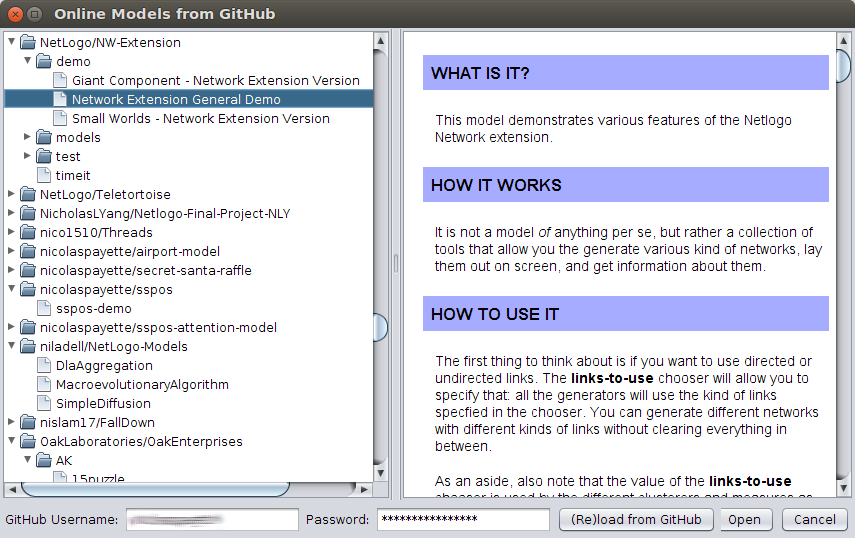
\includegraphics[width=0.75\textwidth]{screenshot.png}
  \caption{A screenshot of the ``Online Models'' dialogue inside NetLogo.}
  \label{fig:screenshot}
\end{figure}

\section{Version control systems and obstacles to their use}

Simply put, a version control system is ``a system that records changes to a file or set of files over time so that you can recall specific versions later.'' \cite{chacon_pro_2014} This is useful for a lone programmer tracking the progress of a personal project, but it borders on essential when multiple programmers are trying to collaborate on a common project. Version control systems track what was changed when by whom. They also offer ways to resolve ``merge conflicts'' when multiple people tried to change the same thing at the same time.

To fully leverage the power of version control systems, the files dealt with must be plain text files: this allows the user to see exactly what was changed in each file (by herself or someone else) from one version to another and to make decisions accordingly. The need for plain text files for version control to be effective might explain part of the academic community's reluctance to embrace it: after all, the quintessential academic artefact today is arguably a paper written in Microsoft Word, a piece of software infamous for the inscrutability of its file format\footnote{The possibility of using version control systems with \LaTeX{} is one of the advantages it has over Word.}. Users of Word somehow manage to collaborate using the ``track changes'' feature, but their proficiency with this feature is not transferable to something like an agent-based model written in NetLogo.

The learning curve that comes with the use of version control systems might be the single biggest impediment to their adoption. Some graphical user interfaces exist for them, but most version control systems still require occasional trips to the command line: a land of text and keyboard shortcuts that can seem daunting compared to icons and mouse clicks. The conceptual model associated with some version control systems also requires some getting used to. In Git, for example, the underlying model is a directed acyclic graph of \emph{commits}, with \emph{branches} and \emph{merges}, and changes move from your \emph{working directory} to the \emph{repository} via a \emph{staging area}. These concepts, unknown to most users, need to be added on top of a simple understanding of the computer's file system. Version control also comes with a deeper conceptual shift: you realize that the artefacts that you are dealing with are not just mutating over time, they carry their whole history with them. Once you have made that conceptual shift, the idea of working without version control becomes unbearable.

The NetLogo user experience, by virtue of its ``low threshold, high ceiling'' philosophy, has some elements in common with a WYSIWYG\footnote{``What You See Is What You Get.''} tool like Word: your model is (usually) a self-contained file that includes its visual interface in addition to its documentation and code. This is both a blessing and a curse. It allows users to immerse themselves in a friendly environment with everything they need at their fingertips, without having to juggle multiple heterogeneous external tools. It does mean, however, that unless they are already familiar and comfortable with them, they tend to forfeit the power of these tools.

One of the purposes of the ``Online Models'' tool that we are proposing is admittedly to act as a Trojan horse: by making NetLogo models stored on GitHub easily discoverable and loadable from \emph{within} NetLogo, we give users an incentive to integrate version control and collaboration using Git and GitHub through their whole workflow.

\section{Alternatives for sharing and collaborating on models}

Model description protocols like ODD \cite{grimm_standard_2006,grimm_odd_2010} are useful, but not sufficient. Models should not only be described, they should be shared. It is the only way to ensure that results can be reproduced and checked. It is also the best way to increase the chances that other people use and improve the model.

The closest thing to an adopted standard for sharing models in the agent-based modelling community is the OpenABM website of the CoMSES network\cite{noauthor_comses_nodate}. At the time of writing, it hosts a library of 484 models with their associated documentation, sometimes giving access to multiple versions of the models. It also offers a peer review service where models are checked for ``structural completeness and fulfilling community standards.'' As long as the sole purpose is to make models publicly available, a site like\footnote{The ``User Community Models'' section of the Center for Connected Learning's website \cite{noauthor_netlogo_nodate} plays a similar role, and non-ABM-specific scientific archiving sites\cite{noauthor_dataverse_nodate,noauthor_open_nodate,noauthor_zenodo_nodate} can also be used for that purpose.} OpenABM is perfectly adequate.

Our goal, however, should not only be to share models, but also to collaborate on them. The NetLogo Modeling Commons \cite{lerner_connected_2010,lerner_agent-based_2014} goes many steps beyond simple sharing. Its features are too numerous to be exhaustively listed here, but it allows users to modify and comment on each other's models and to (crudely) compare model versions. The fact that it allows models to be uploaded from within NetLogo is also a big advantage.

There are two ways in which the Modeling Commons fall short, though. The first is that model discovery is not integrated into NetLogo. If you want to look at shared models, you have to open your browser, navigate to the website, use their search tools to find an interesting model, download it, save it locally, and then open it in NetLogo. In our ``Online Models'' tool, by contrast, new models are accessible in just a few clicks or keystrokes, without ever leaving the NetLogo interface. The second downside is that the Modeling Commons only work for NetLogo models. GitHub and Git, by contrast, are language agnostic and bring together most of the open-source development community. It means that models developed on GitHub are potentially discoverable by a lot more people. It also means that the proficiency acquired with Git can be extended to other project artefacts (e.g., analysis code in R, papers in \LaTeX, etc.).

\section{Future developments}

The tool, in its current state of development\footnote{The tool is currently being developed in a fork of the NetLogo codebase\cite{payette_netlogo_2018}, but the plan is to make it available as a plugin that can easily be installed in the official distribution of NetLogo.}, is pretty straightforward: it's very much like NetLogo's Models Library dialogue, except that the models are stored online on GitHub. A browsable tree appears on the right and the currently selected model's ``Info tab'' appears on the left (see, again, \cref{fig:screenshot}). If you click on the ``Open'' button, the model is loaded into NetLogo. GitHub users don't need to do anything out of the ordinary for their models to appear in the dialogue: as soon as the model is pushed to a public repository, it shows up in the dialogue.

We believe this sharing/discovery-enabling feature to be sufficient to justify the existence of the tool, but it is the potential for further integration with GitHub that makes it exciting. Here are a few features that could be made easily accessible from within the NetLogo interface:

\begin{itemize}
  \item Uploading the current model to a new repository on GitHub;
  \item Committing changes to the current model and pushing them to GitHub;
  \item ``Forking'' (i.e., making a modifiable copy of) someone else's model;
  \item Opening ``pull requests'' (i.e., proposing changes) for someone else's model;
  \item Showing the differences between two versions of a model in the code tab.
\end{itemize}

Taken together, these features would significantly lower the barrier to the adoption of version control for NetLogo models. Combined with the incentive of making a model easily available to all users of our tool, this might help to kickstart the adoption of open collaboration practices for agent-based modellers. In a not so distant future, perhaps our community will also be able to boast of collective achievements on the level of the greatest open-source successes.

\bibliography{online_models}

\end{document}
